\documentclass{standalone}
\usepackage{xcolor}
\usepackage{tikz}
\usetikzlibrary{positioning, shapes.multipart, calc, graphs, graphs.standard}
\begin{document}
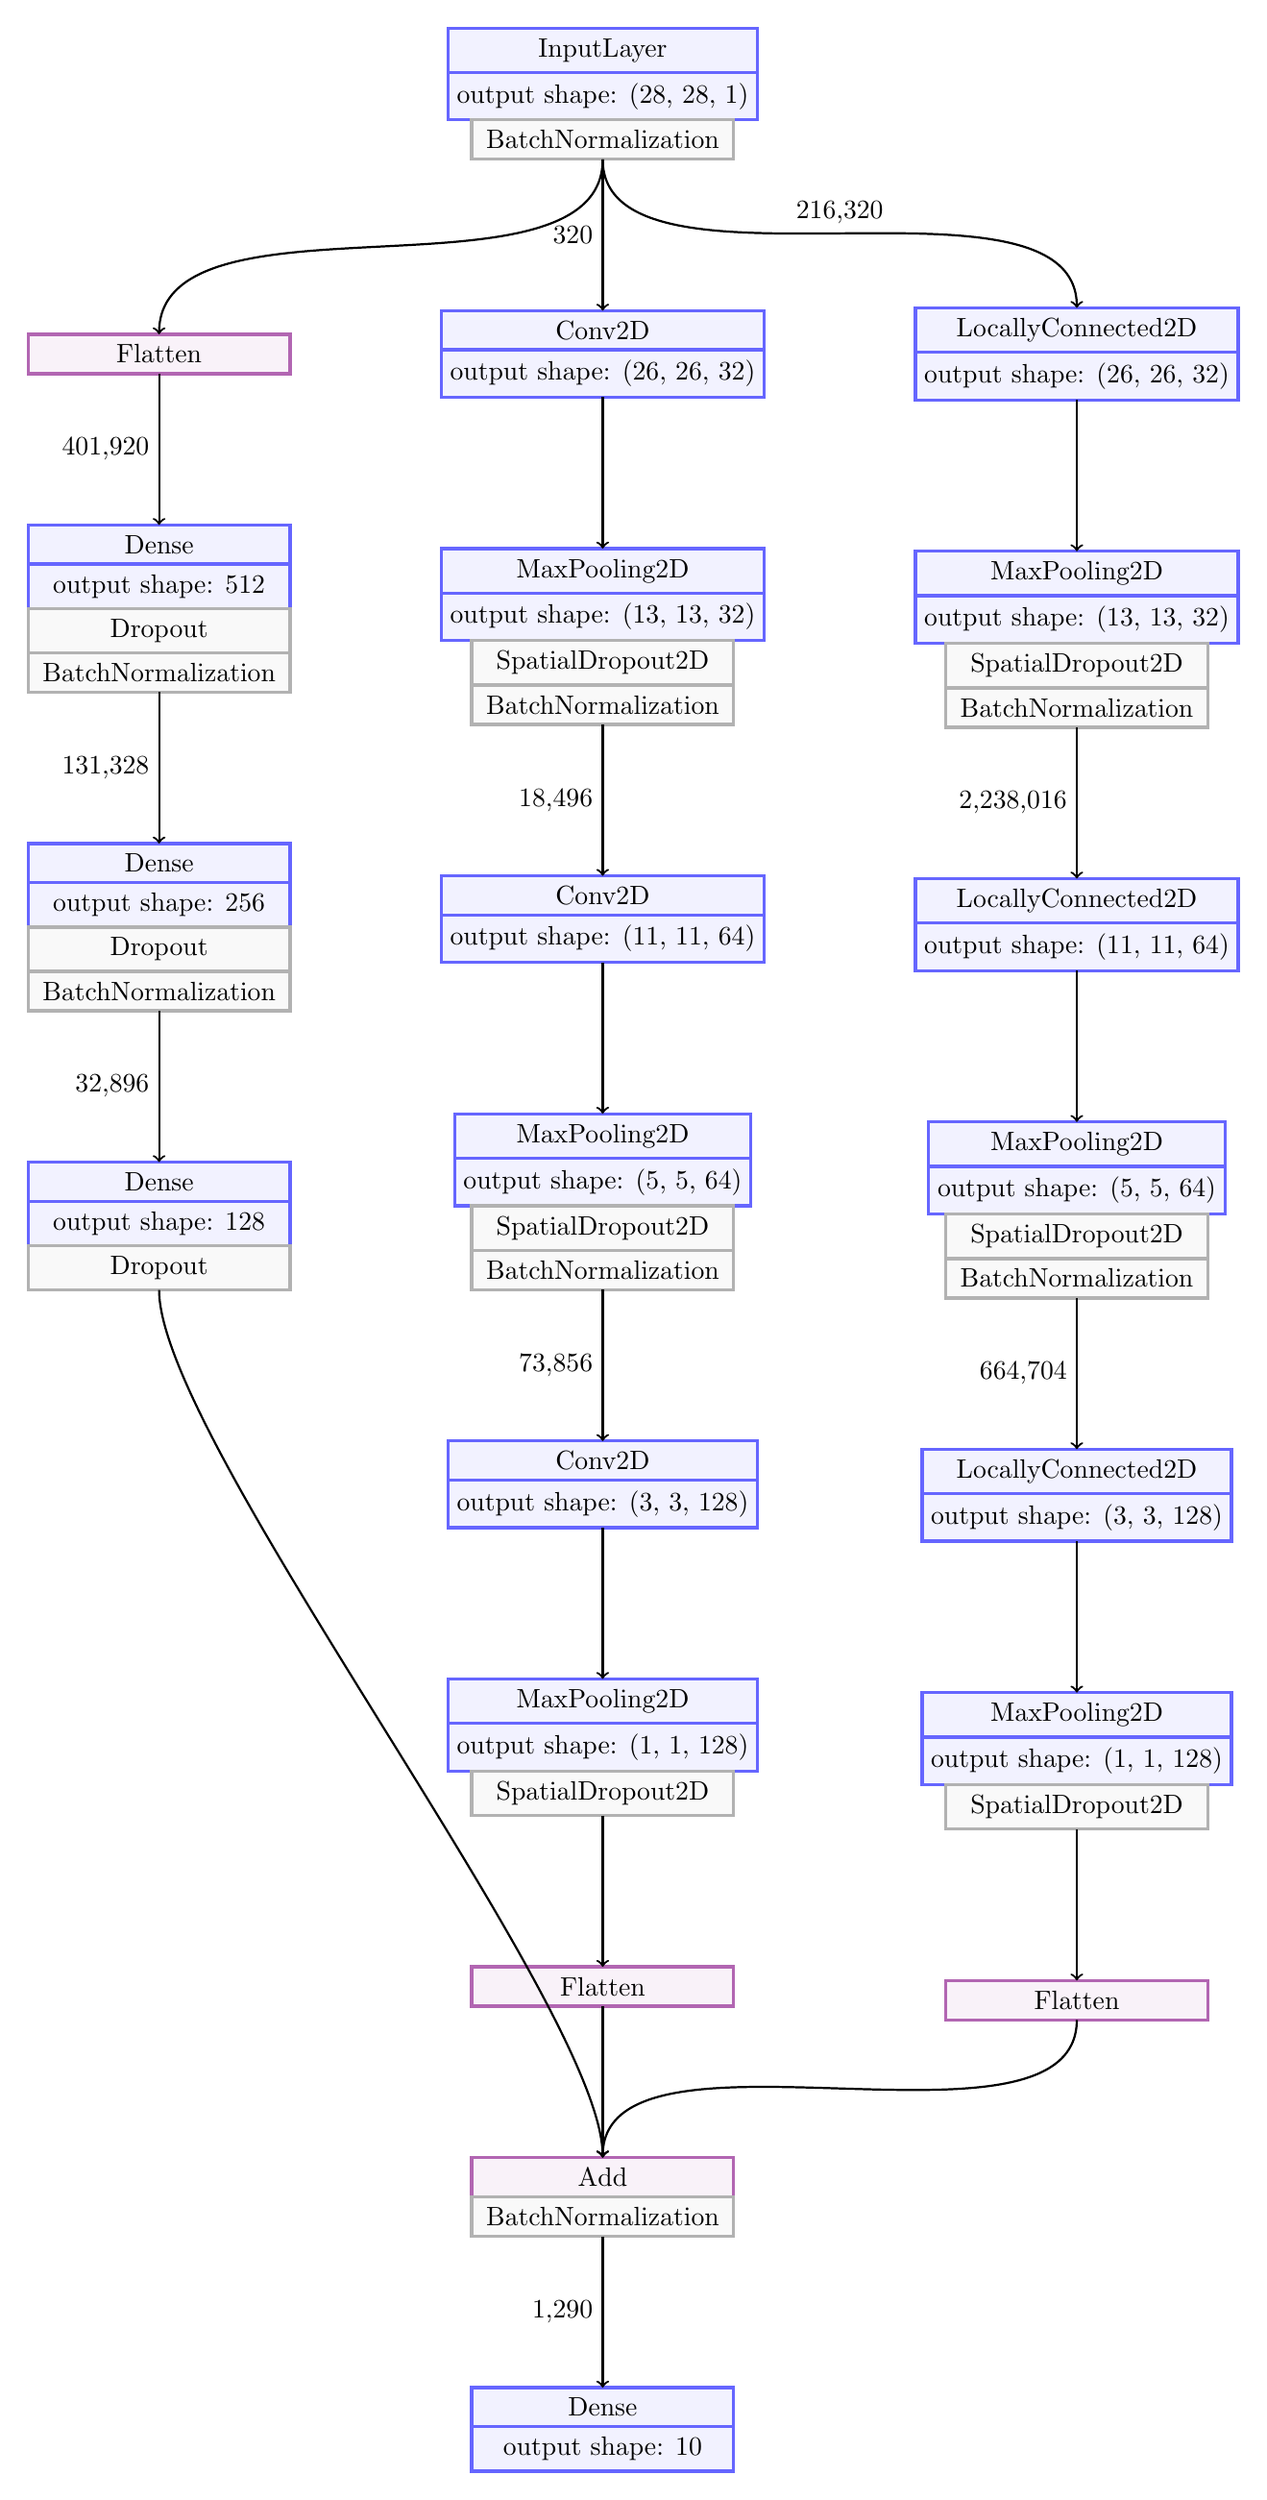
\begin{tikzpicture}
[trainable_node/.style={rectangle split,rectangle split ignore empty parts,very thick,rectangle split parts=2,draw=blue!60,fill=blue!5,minimum width={width("Batch Normalisation") + 8pt},node distance=2,outer sep=0pt},utility_node/.style={rectangle split,rectangle split ignore empty parts,very thick,rectangle split parts=2,draw=gray!60,fill=gray!5,minimum width={width("Batch Normalisation") + 8pt},node distance=2,outer sep=0pt},operation_node/.style={rectangle split,rectangle split ignore empty parts,very thick,rectangle split parts=2,draw=violet!60,fill=violet!5,minimum width={width("Batch Normalisation") + 8pt},node distance=2,outer sep=0pt},default_edge/.style={thick,out=-90,in=90,out distance=2cm,in distance=2cm},default_label/.style={midway,auto}]
\node[trainable_node] [] (input_2) {InputLayer\nodepart{two}output shape: (28, 28, 1)};

\node[utility_node] [below=of input_2,yshift=2cm] (batch_normalization_10) {BatchNormalization};

\node[trainable_node] [below=of batch_normalization_10] (conv2d_3) {Conv2D\nodepart{two}output shape: (26, 26, 32)};

\node[trainable_node] [below=of batch_normalization_10,right=of conv2d_3] (locally_connected2d_3) {LocallyConnected2D\nodepart{two}output shape: (26, 26, 32)};

\node[trainable_node] [below=of conv2d_3] (max_pooling2d_9) {MaxPooling2D\nodepart{two}output shape: (13, 13, 32)};

\node[trainable_node] [below=of locally_connected2d_3] (max_pooling2d_12) {MaxPooling2D\nodepart{two}output shape: (13, 13, 32)};

\node[utility_node] [below=of max_pooling2d_9,yshift=2cm] (spatial_dropout2d_9) {SpatialDropout2D};

\node[utility_node] [below=of max_pooling2d_12,yshift=2cm] (spatial_dropout2d_12) {SpatialDropout2D};

\node[utility_node] [below=of spatial_dropout2d_9,yshift=2cm] (batch_normalization_11) {BatchNormalization};

\node[utility_node] [below=of spatial_dropout2d_12,yshift=2cm] (batch_normalization_13) {BatchNormalization};

\node[operation_node] [below=of batch_normalization_10,left=of conv2d_3] (flatten_6) {Flatten};

\node[trainable_node] [below=of batch_normalization_11] (conv2d_4) {Conv2D\nodepart{two}output shape: (11, 11, 64)};

\node[trainable_node] [below=of batch_normalization_13] (locally_connected2d_4) {LocallyConnected2D\nodepart{two}output shape: (11, 11, 64)};

\node[trainable_node] [below=of flatten_6] (dense_4) {Dense\nodepart{two}output shape: 512};

\node[trainable_node] [below=of conv2d_4] (max_pooling2d_10) {MaxPooling2D\nodepart{two}output shape: (5, 5, 64)};

\node[trainable_node] [below=of locally_connected2d_4] (max_pooling2d_13) {MaxPooling2D\nodepart{two}output shape: (5, 5, 64)};

\node[utility_node] [below=of dense_4,yshift=2cm] (dropout_3) {Dropout};

\node[utility_node] [below=of max_pooling2d_10,yshift=2cm] (spatial_dropout2d_10) {SpatialDropout2D};

\node[utility_node] [below=of max_pooling2d_13,yshift=2cm] (spatial_dropout2d_13) {SpatialDropout2D};

\node[utility_node] [below=of dropout_3,yshift=2cm] (batch_normalization_15) {BatchNormalization};

\node[utility_node] [below=of spatial_dropout2d_10,yshift=2cm] (batch_normalization_12) {BatchNormalization};

\node[utility_node] [below=of spatial_dropout2d_13,yshift=2cm] (batch_normalization_14) {BatchNormalization};

\node[trainable_node] [below=of batch_normalization_15] (dense_5) {Dense\nodepart{two}output shape: 256};

\node[trainable_node] [below=of batch_normalization_12] (conv2d_5) {Conv2D\nodepart{two}output shape: (3, 3, 128)};

\node[trainable_node] [below=of batch_normalization_14] (locally_connected2d_5) {LocallyConnected2D\nodepart{two}output shape: (3, 3, 128)};

\node[utility_node] [below=of dense_5,yshift=2cm] (dropout_4) {Dropout};

\node[trainable_node] [below=of conv2d_5] (max_pooling2d_11) {MaxPooling2D\nodepart{two}output shape: (1, 1, 128)};

\node[trainable_node] [below=of locally_connected2d_5] (max_pooling2d_14) {MaxPooling2D\nodepart{two}output shape: (1, 1, 128)};

\node[utility_node] [below=of dropout_4,yshift=2cm] (batch_normalization_16) {BatchNormalization};

\node[utility_node] [below=of max_pooling2d_11,yshift=2cm] (spatial_dropout2d_11) {SpatialDropout2D};

\node[utility_node] [below=of max_pooling2d_14,yshift=2cm] (spatial_dropout2d_14) {SpatialDropout2D};

\node[trainable_node] [below=of batch_normalization_16] (dense_6) {Dense\nodepart{two}output shape: 128};

\node[operation_node] [below=of spatial_dropout2d_11] (flatten_4) {Flatten};

\node[operation_node] [below=of spatial_dropout2d_14] (flatten_5) {Flatten};

\node[utility_node] [below=of dense_6,yshift=2cm] (dropout_5) {Dropout};

\node[operation_node] [below=of flatten_4] (add_1) {Add};

\node[utility_node] [below=of add_1,yshift=2cm] (batch_normalization_17) {BatchNormalization};

\node[trainable_node] [below=of batch_normalization_17] (dense_7) {Dense\nodepart{two}output shape: 10};

\draw[->, default_edge] (batch_normalization_10) to node [default_label] {320} (conv2d_3);
 
\draw[->, default_edge] (batch_normalization_10) to node [default_label] {216,320} (locally_connected2d_3);
 
\draw[->, default_edge] (batch_normalization_10) to node [default_label] {} (flatten_6);
 
\draw[->, default_edge] (conv2d_3) to node [default_label] {} (max_pooling2d_9);
 
\draw[->, default_edge] (locally_connected2d_3) to node [default_label] {} (max_pooling2d_12);
 
\draw[->, default_edge] (batch_normalization_11) to node [default_label] {18,496} (conv2d_4);
 
\draw[->, default_edge] (batch_normalization_13) to node [default_label] {2,238,016} (locally_connected2d_4);
 
\draw[->, default_edge] (flatten_6) to node [default_label] {401,920} (dense_4);
 
\draw[->, default_edge] (conv2d_4) to node [default_label] {} (max_pooling2d_10);
 
\draw[->, default_edge] (locally_connected2d_4) to node [default_label] {} (max_pooling2d_13);
 
\draw[->, default_edge] (batch_normalization_15) to node [default_label] {131,328} (dense_5);
 
\draw[->, default_edge] (batch_normalization_12) to node [default_label] {73,856} (conv2d_5);
 
\draw[->, default_edge] (batch_normalization_14) to node [default_label] {664,704} (locally_connected2d_5);
 
\draw[->, default_edge] (conv2d_5) to node [default_label] {} (max_pooling2d_11);
 
\draw[->, default_edge] (locally_connected2d_5) to node [default_label] {} (max_pooling2d_14);
 
\draw[->, default_edge] (batch_normalization_16) to node [default_label] {32,896} (dense_6);
 
\draw[->, default_edge] (spatial_dropout2d_11) to node [default_label] {} (flatten_4);
 
\draw[->, default_edge] (spatial_dropout2d_14) to node [default_label] {} (flatten_5);
 
\draw[->, default_edge] (flatten_4) to node [default_label] {} (add_1);
 
\draw[->, default_edge] (flatten_5) to node [default_label] {} (add_1);
 
\draw[->, default_edge] (dropout_5) to node [default_label] {} (add_1);
 
\draw[->, default_edge] (batch_normalization_17) to node [default_label] {1,290} (dense_7);
 \end{tikzpicture}\end{document}